\documentclass[11pt,a4paper]{article}
\usepackage{cite}
\usepackage{apalike}
\usepackage{amsmath}
\usepackage{amsfonts}
\usepackage{amssymb}
\usepackage{makeidx}
\usepackage{graphicx}
\usepackage{wrapfig}
\usepackage{enumerate}
\usepackage{pdfpages}
\usepackage{tocloft}
\usepackage{setspace}
\usepackage{mathtools}
\usepackage{hyperref}
\definecolor{linkcolour}{rgb}{0,0.2,0.6} % Link color
\hypersetup{colorlinks,breaklinks,urlcolor=linkcolour,linkcolor=linkcolour, citecolor=linkcolour}

\usepackage[left=2cm,right=2cm,top=2cm,bottom=2cm]{geometry}

\usepackage{xcolor}

\usepackage{fontspec}
\setmainfont{Cambria}

\usepackage{caption}
\captionsetup[figure]{font=small, labelfont={bf}}
\captionsetup[table]{font=small, labelfont={bf}}

\usepackage{float}
\usepackage{multirow}
\usepackage{longtable}

\usepackage[nottoc]{tocbibind}
\setcounter{tocdepth}{4}
\setcounter{secnumdepth}{4}

% FOr subfigure
\usepackage{caption}
\usepackage{subcaption}

\newcommand{\spa}{\vspace{1.25em}}
\newcommand{\noi}{\noindent}
\def\dul#1{\underline{\underline{#1}}}
\def\cpt#1#2{{\begin{center}\small\textbf{\textcolor{blue}{Figure #1:}} #2\end{center}}}

% for dots in the content
\usepackage{tocloft}
\renewcommand{\cftsecleader}{\cftdotfill{\cftdotsep}}

\begin{document}
	\begin{titlepage} 
		\begin{center}
		\large{MINI PROJECT 2}\\
		% \vspace{1em}
		\large {COGS 209 Scientific Data Analysis and Statistical Learning}
		\vspace{3em}
		
		\rule{0.9\linewidth}{0.5mm} \\[0.4cm]
	    {\Large{\bfseries{Development of a chemotyping strategy for consumer \textit{Cannabis sativa}}}} \\
	    \rule{0.9\linewidth}{0.5mm} \\[3 em]	
	    
	    \vspace{5em}

	    Lead Author: Michaela Cullum-Doyle\\

	    \vspace{1em}

	    Co-Authors: Morgan Fitzgerald, Sowmya Manojna, Vanessa Martin \\

		\vspace{25em}

		University of California, San Diego
		
		\vspace{5em}    
	    
    	% \includegraphics[scale = 0.09]{images/iitmlogo.png}
		\end{center}
	\end{titlepage}

{\hypersetup{linkcolor=black}
 \tableofcontents}
\break

\section{Introduction}
\subsection{Background}
Cannabis is a drug cultivated from the Cannabis plant that is known for its psychoactive and medicinal properties. In the 20th century, the recreational consumption of cannabis became widespread given its ability to promote relaxation and euphoria. However, in the 1970s, the US deemed cannabis to be a Schedule 1 controlled substance and its use is illegal in most countries (\cite{united1970comprehensive}, enacted October 27, 1970). Despite its recreational use, recent clinical studies have shown that cannabis has medicinal use to treat and alleviate symptoms of diseases such as helping patients with HIV infection gain weight \cite{hill2019medical}. Recently, laws have gone into effect that has permitted the use of cannabis for both medicinal and recreational uses in numerous states in the United States, allowing the demand for cannabis to increase.
\\

\noi
Cannabis has a complex chemical composition that is dependent on factors such as strain, processing methods, and genetic modification. The most well-known chemical compounds in cannabis are cannabinoids, specifically delta-9-tetrahydrocannabinol (THC) and cannabidiol (CBD) which interact with our endocannabinoid system. THC is the primary psychoactive compound in cannabis and has therapeutic properties such as increasing appetite, reducing nausea, and pain relief. CBD is non-psychoactive and has promising medical applications such as anxiety relief, anti-inflammatory, and anti-epileptic \cite{gonccalves2020terpenoids}. In addition to cannabinoids, another important chemical compound found in cannabis is terpenes which are aromatic compounds that work synergistically with cannabinoids \cite{russo2011taming}. There are over 100 different types of terpenes such as mycrene, limonene and the concentration and composition of terpenes varies in each strain of cannabis \cite{booth2019terpenes}. The chemical composition of cannabis can be influence by the region it is sourced from. Factors such as climate, cultivation practices, soil composition and genetic variation can greatly influence the cannabinoid and terpene composition in cannabis \cite{smith2022phytochemical}. It is important to understand the chemical composition that underlies cannabis because it can provide valuable information regarding the potency of the product for consumer safety, efficacy, and medicinal usage. However, the current practice for the classification of cannabis is by the strain of the plant species, which fails to account for the underlying chemical makeup.\\
 
\noi
In this study, we aim to classify strains of cannabis by their chemical composition and regional distribution using publicly available cannabis chemical profiles from \cite{smith2022phytochemical}. We looked at the chemical phenotype of almost 90,000 commercially available cannabis-derived products and employed clustering algorithms Density- Based Spatial Clustering of Applications with Noise (DBSCAN) and K-means to identify clusters of cannabis based on their chemical concentrations of both cannabinoids and terpenes and visualized our findings using Uniform Manifold Approximation and Projections (UMAPs). Clustering algorithms such an DBSCAN and K-means aim to cluster data based of their similar characteristics and are unsupervised learning methods that only relies on the characteristics of the data. Based on our preliminary findings, we hypothesized that K-means might outperform DBSCAN in cannabis clustering as the clusters identified by K-means looked similar to historial cannabis strain data. However, a more robust comparison between clustering methods was necessary. Overall, this study will provide a comparison of two clustering methods for the classification of cannabis based on multiple strain properties, and could aid in future strain identification. 



\section{Methods}
\subsection{Data}
\subsubsection{Description}
In this analysis, we leveraged a publicly available cannabis chemical profile dataset from the article by \cite{smith2022phytochemical}. The dataset can be publicly accessed from GitHub: \url{https://github.com/cjsmith015/phytochemical-diversity-cannabis/tree/main/data}. The dataset comprises cannabis strain specific information including region the sample was sourced from, strain information of the sample and the chemical composition of the sample.


\subsubsection{Preprocessing}
The dataset was loaded from GitHub and only the columns relevant to the analysis are selected. This selected dataset was used for all subsequent processing steps. The cannabinoid and terpene data are separately normalized, so as to account for product based variations as highlighted in the project proposal. As the dataset was large, we opted to drop all entries with missing data.\\

\subsection{Exploratory Data Analysis}
Exploratory Data Analysis (EDA) was performed on the dataset. Correlations (Pearson's) were obtained and analyzed for any trends. Some observations that we can draw from the correlation plot in \autoref{fig:corr_plot} is as follows:

\begin{figure}[H]
	\centering
	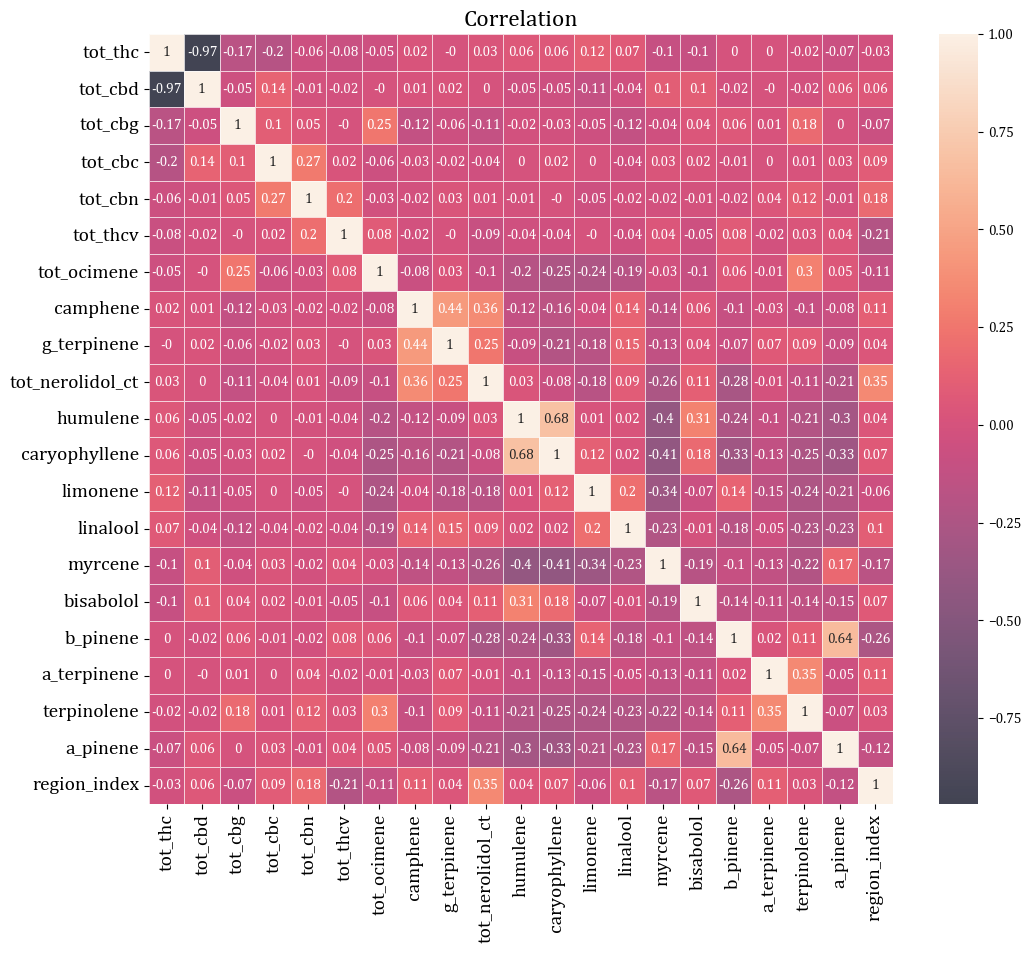
\includegraphics[scale=0.5]{images/corr.png}
	\caption{Correlation Analysis on the dataset.}
	\label{fig:corr_plot}
\end{figure}

\begin{itemize}
	\itemsep0em
	\item \texttt{tot\_cbd} and \texttt{tot\_thc} are highly negatively correlated
	\item \texttt{a\_pinene} and \texttt{b\_pinene} are highly positively correlated
	\item \texttt{caryophyllene} and \texttt{humulene} are highly positively correlated
	\item \texttt{camphene} and \texttt{g\_terpinene} are positively correlated
	\item \texttt{caryophyllene} and \texttt{myrcene} are negatively correlated
	\item \texttt{tot\_nerolidol\_ct} is positively correlated with the value of the region. The region values correspond to `AK', `CA', `FL', `MI', `OR', `WA', in that order. Higher values are assigned to WA, OR and MI. Hence, the positive correlation implies that the cannabis from these states generally tend to have greater fragrance.

\end{itemize}
% 
\subsection{Dimensionality Reduction}
In addition to employing Principal Component Analysis (PCA) for clustering, we decided to incorporate UMAP as a complementary dimensionality reduction technique. While PCA captures linear relationships, we suspected that our dataset contained non-linearities that could impact the clustering results. UMAP, being a non-linear dimensionality reduction method, preserves both local and global structure of the data, making it suitable for capturing complex patterns. By applying UMAP to the entire dataset, we aimed to uncover intricate relationships and visualize the non-linear structure present within the data. This approach allowed us to gain a holistic understanding of the data points, facilitating the detection of global patterns and dependencies that might have been overlooked by linear techniques alone. Furthermore, by leveraging UMAP, we were able to incorporate additional perspectives by coloring the visualization based on Principal Components (PCs), regions, and dominant terpenes, providing a multi-faceted analysis of the dataset.


\subsection{Clustering analysis}
\subsubsection{DBSCAN}
In our clustering analysis, we utilized the DBSCAN algorithm on the reduced-dimensional data obtained through UMAP. Unlike traditional clustering methods like K-means, DBSCAN does not require a priori specification of the number of clusters. Instead, it defines clusters based on the density of data points in the feature space. DBSCAN identifies core points that have a sufficient number of neighboring points within a specified distance threshold. It then expands the clusters by including directly reachable points. Any points that do not meet the density criteria are considered noise or outliers. For the clustering analysis, we used the default parameters of the DBSCAN algorithm. Our objective was to leverage the algorithm's capability to discover natural clusters within the cannabis dataset based on the extracted features. The advantage of using DBSCAN in this analysis lies in its ability to capture clusters of different densities and shapes, making it well-suited for identifying cannabis strain categories based on their chemical profiles. By analyzing the proximity and density of data points in the feature space, DBSCAN can reveal meaningful groupings that may not be apparent with traditional clustering algorithms. \\

\noi
Once the clusters were obtained through DBSCAN, the next step involved visualizing and exploring the results using UMAP. Each data point was assigned a color or marker based on its cluster membership obtained from DBSCAN. This visualization provided a comprehensive understanding of the spatial distribution of the clusters in the reduced-dimensional space. By plotting the clusters onto UMAP, we were able to visually assess the separation and proximity of different clusters. This visualization helped identify potential overlaps or distinct regions in the data, providing insights into grouping patterns and similarities between different cannabis strains. Such visual exploration played a crucial role in interpreting and validating the clustering results obtained from DBSCAN.

\subsubsection{K-Means}
After applying the DBSCAN algorithm to identify clusters in the cannabis dataset, we conducted an additional analysis using the K-means clustering algorithm. K-means is a widely used method that partitions the data into a predefined number of clusters by minimizing the within-cluster sum of squares distance. The purpose of employing K-means was twofold. Firstly, it allowed us to gain further insights into the dataset and validate the results obtained from DBSCAN. By creating a new set of clusters based on the K-means algorithm's criterion, we could compare and contrast the clustering outcomes with those obtained from DBSCAN. It is important to note that K-means requires the specification of the number of clusters in advance. The choice of the number of clusters can significantly impact the interpretation of the results. Setting the appropriate number of clusters ensures that each cluster represents a distinct group or pattern within the data.\\

\noi
To visualize the K-means clustering results, we also plotted the clusters onto UMAP. Each data point was assigned a specific color or marker based on its cluster membership derived from the K-means algorithm. This visual representation facilitated the assessment of the separation and proximity of the K-means clusters. It provided an intuitive understanding of the different groupings present in the cannabis dataset and aided in identifying potential patterns or relationships within the data. By incorporating both DBSCAN and K-means clustering techniques, along with UMAP for visualization, we aimed to comprehensively analyze the cannabis dataset from different perspectives. This multifaceted approach allowed us to uncover underlying patterns, validate clustering outcomes, and gain a deeper understanding of the distinct groups and relationships within the dataset.

\subsubsection{Comparitive Analysis}
In addition to the DBSCAN and K-means clustering methods, we conducted a detailed comparison of the resulting cluster profiles to further analyze the cannabis dataset. Profile plots were utilized to visualize and compare the characteristics of the clusters obtained from both methods. For each clustering approach, we generated profile plots that depicted the distribution of chemical profiles across the identified clusters. These plots provided a comprehensive overview of the variations in chemical composition within each cluster, allowing us to assess the distinctiveness and coherence of the clusters.\\

\noi
To perform the comparison, we carefully examined the profile plots side by side, focusing on the similarities and differences in the distribution patterns of chemical constituents across the clusters. This enabled us to identify any overlapping or distinct clusters, as well as assess the degree of agreement or disagreement between the two clustering methods. By scrutinizing the profile plots, we could gain insights into the consistency and stability of the cluster assignments. Consistent patterns across both methods would indicate robust and reliable clusters, while discrepancies would highlight areas for further investigation or potential refinements in the clustering analysis. Furthermore, the comparison of profile plots allowed us to evaluate the effectiveness of each clustering method in capturing the underlying chemotypic similarities and differences. We could discern whether certain clusters exhibited similar profiles across both methods, suggesting a strong agreement, or if there were notable divergences, indicating potential limitations or biases inherent to a particular clustering approach. The profile plot comparison served as a methodical and data-driven assessment of the clustering outcomes, providing a comprehensive understanding of the clustering patterns and aiding in the interpretation and validation of the results. It offered valuable insights into the similarities and dissimilarities between clusters identified by DBSCAN and K-means, enriching the overall analysis and contributing to a robust characterization of the cannabis dataset.

\section{Results \& Comparisons}
The final preprocessed dataset used in all our analysis consisted of 26,033 samples and 20 different strain characteristics.

\subsection{Principal Component Analysis}
To gain insights into the underlying structure and variability of the cannabis dataset, we applied PCA on the dataset. The results of the PCA analysis are summarized in \autoref{fig:pca_variance}, which illustrates the explained variance ratio across principal components. The plot showcases the relationship between the principal component number and the percentage of variance explained. Notably, out of the 19 principal components computed, the 19th component exhibited a variance of zero, indicating no contribution to the overall variability. In contrast, PC 1 demonstrated a higher value, surpassing 0.14 on the y-axis. This suggests that PC 1 plays a crucial role in explaining a substantial portion of the dataset's variability. Therefore, PC 1 captures the most dominant patterns or characteristics within the cannabis dataset far above the subsequent components. The findings from the PCA analysis offer valuable information regarding the relative importance of each principal component.\\

\noi
The distribution of the cannabis dataset in the PC1-PC2 space was examined to gain insights into the underlying patterns and relationships. Figure 2 presents the results of this analysis, where \autoref{fig:tot_thc} displays the dataset distribution colored by the amount of \texttt{tot\_thc}, and \autoref{fig:tot_cbd} represents the dataset distribution colored by the amount of \texttt{tot\_cbd}. The plots provide a visual representation of how the samples are organized based on the levels of THC and CBD content, respectively. Notably, PCs 1 and 2 were found to differentiate samples based on both \texttt{tot\_thc} and \texttt{tot\_cbd}, albeit with gradations in opposite directions. The significance of this observation remains uncertain and may be influenced by factors such as unit sums or complex interactions within the dataset. These findings from the PCA analysis contribute to our understanding of the variability and relationships among the cannabis strains in terms of their chemical profiles.

\subsection{UMAP Clustering}
To explore the structure and relationships within the cannabis dataset, we employed the UMAP visualization technique. \autoref{fig:umap_n_neigh} displays UMAP plots with varying choices for the number of neighbors (\texttt{n\_neighbors}) parameter. When \texttt{n\_neighbors} was set to 10, the UMAP plot revealed a scattered and indistinct pattern. However, as the number of neighbors increased to 15, slight improvements in the clustering structure became apparent, suggesting the emergence of underlying patterns. Surprisingly, increasing the number of neighbors beyond 45 or 60 did not significantly refine the UMAP visualization (\autoref{fig:umap_n_neigh}). These findings underscored the critical role of the \texttt{n\_neighbors} parameter in capturing meaningful structures within the cannabis dataset and emphasized the importance of careful parameter selection for informative visualizations.

\subsubsection{UMAP Visualization of Clusters}
In our analysis focused on classifying cannabis strains, we utilized UMAP to visualize the dataset, coloring the UMAP plot based on the values of PC1. \autoref{fig:umap_pc1} displayed the UMAP visualization colored by the first principal component (PC1), revealing the presence of distinct clusters in the dataset. While the boundaries between these clusters were not entirely well-defined, emerging patterns and relationships indicated the existence of distinct subgroups or trends within the data. The observed clusters suggested potential substructures and underlying patterns that warranted further investigation and analysis of these cannabis clusters. Interestingly, the UMAP plots where colors were assigned based on the values of the second and third principal components (PC2 and PC3) displayed a dominant and uniform color throughout, indicating that PC2 and PC3 did not capture significant variation or distinct patterns in the dataset. As expected based on previous mentioned PCA results, this suggested limited relevance of PC2 and PC3 in explaining the underlying structure of the cannabis strains dataset, possibly due to weaker correlation or redundancy with other principal components. \\

\noi
Applying UMAP as a dimensionality reduction technique, we visualized the dataset with colors assigned based on the dominant terpene present in each sample \autoref{fig:umap_terpene}. The resulting UMAP plot displayed a diverse distribution of colors, indicating the presence of various dominant terpenes within the dataset. Notably, the plot exhibited clusters with clear boundaries, suggesting that the dominant terpene plays a significant role in determining the overall composition and grouping of the samples. This finding emphasized the importance of terpene profiles in characterizing cannabis strains and highlighted the potential utility of dominant terpenes as key discriminative factors in strain classification and selection. 

\subsection{Comparative Cluster Analysis}
\subsubsection{DBSCAN}
From the results obtained, as illustrated in \autoref{fig:dbscan}, we can see that DBSCAN was able to identify outlier data points and correctly classify them as noise. In addition to identifying noise, DBSCAN was also able to cluster points that have similar chemical composition such as:
\begin{itemize}
	\itemsep0em
	\item Cluster 1: High concentrations of THC; Moderate concentrations of myrcene; Low concentrations of CBD
	\item Cluster 2: High concentrations of CBD, myrcene and THC
	\item Cluster 3: High concentrations of CBD and myrcene; Low concentrations of THC
	\item Cluster 4: High concentrations of THC and terpinene/terpinolene
\end{itemize}

\subsubsection{K-Means}
The results obtained for k-means varied based on the number of clusters initiated. Hence, the results are discussed in detail, based on the number of clusters initiated.
\paragraph{Number of Clusters: 2}
\begin{itemize}
	\itemsep0em
	\item The model classified most of the data points as belonging to one class. The second class seems to mostly comprise of data points that appear as outliers in the 2D representation of the dataset.
	\item We can see from the chemical composition plot for cluster 1, that the distributions are very similar to the chemical composition distributions obtained for class 1 of DBSCAN. 
	\item As mentioned above, this similarity could arise as the k-means model seems to classify most of the data points as cluster 1. The DBSCAN cluster 1 also comprises 21,201 data points which is a huge fraction of the dataset.
\end{itemize}
\autoref{fig:km2} illustrations pertaining to the results obtained using k-means models initialized with 2 clusters.

\paragraph{Number of Clusters: 4}
\begin{itemize}
	\itemsep0em
	\item From the distribution of the clusters obtained, we can see (to a degree), the centroid based nature of the k-means clustering approach. The data points within each cluster are spatially closer to each other. This is more clear in the individual cluster distribution plots.
	\item The chemical composition of cluster 1 and that of cluster 1 obtained from DBSCAN are similar. However, the concentration of myrcene is higher in the cluster obtained from k-means.
	\item Similarly, the chemical composition of cluster 3 is very similar to the chemical composition of cluster 4 obtained from DBSCAN.
	\item The cluster 2 classified by the model, is found to have a novel chemical composition of high THC and caryophyllene. Similarly, cluster 4 also has a novel chemical composition of high THC and terpinolene, but low concentrations of terpinene.
\end{itemize}
\autoref{fig:km4} illustrations pertaining to the results obtained using k-means models initialized with 4 clusters.

\paragraph{Number of Clusters: 6}
\begin{itemize}
	\itemsep0em
	\item As mentioned in the section above, we can observe the spatial distribution of the clusters. Unlike the model with the number of initial clusters as 4, we can see that there is an overlap of data points belonging to different clusters. This indicates that these clusters could be differentiated based on values from data dimensions higher than 2, which have been plotted here.
	\item The chemical composition of cluster 1 and that of cluster 1 obtained from DBSCAN are similar. However, the concentration of myrcene is higher in the cluster obtained from k-means.
	\item Similarly, the chemical composition of cluster 3 is very similar to the chemical composition of cluster 4 obtained from DBSCAN.
	\item The clusters 2 and 4 identified by this model are very similar to the clusters identified by the k-means model with 4 initial clusters.
	\item The clusters 5 and 6 classified by the model are found to have novel chemical composition. The cluster 5 identified has high THC and nerolidol, while cluster 6 has high THC, myrcene and a-pinene.
\end{itemize}
\autoref{fig:km6} illustrations pertaining to the results obtained using k-means models initialized with 6 clusters.

\paragraph{Number of Clusters: 8}
\begin{itemize}
	\item The chemical composition of clusters 1-4, 6 and 8 are very similar to the chemical composition of clusters obtained previously in DBSCAn or other k-means models.
	\item The clusters 5 and 7 classified by the model have novel chemical composition. The cluster 5 identified has high THC, g-terpinene, camphene and nerolidol, while cluster 7 has low THC, high THCV, myrcene and caryophyllene.
\end{itemize}
\autoref{fig:km8} illustrations pertaining to the results obtained using k-means models initialized with 8 clusters.

\section{Result Visualization}
\begin{figure}[H]
	\centering
	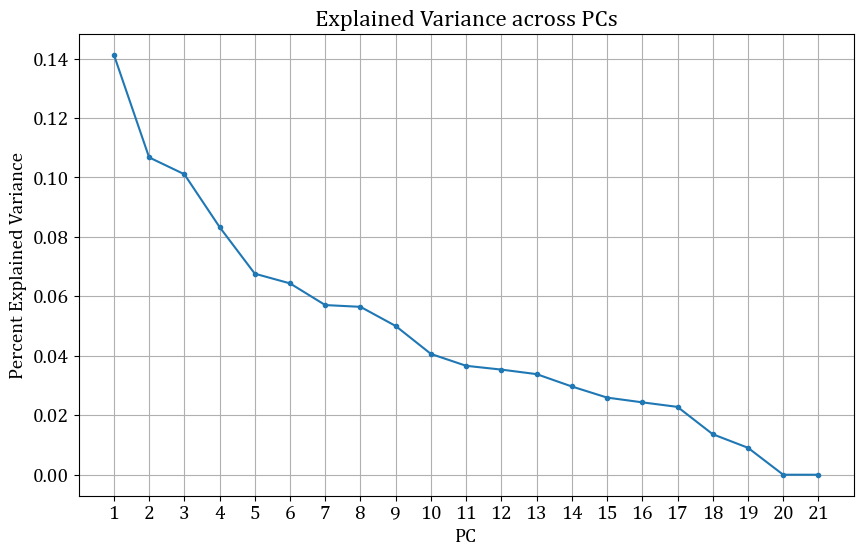
\includegraphics[scale=0.5]{images/pc_variance.png}
	\caption{Explained Variance Ratio by Principal Components.} %The relationship between the principal component number on the x-axis and the percentage of variance explained on the y-axis. A total of 19 principal components were computed, with the 19th component being zero, indicating no contribution to the variance. The explained variance of PC 1 surpassed 0.14.}
	\label{fig:pca_variance}
\end{figure}


\begin{figure}[H]
     \centering
     \begin{subfigure}[b]{0.475\textwidth}
         \centering
         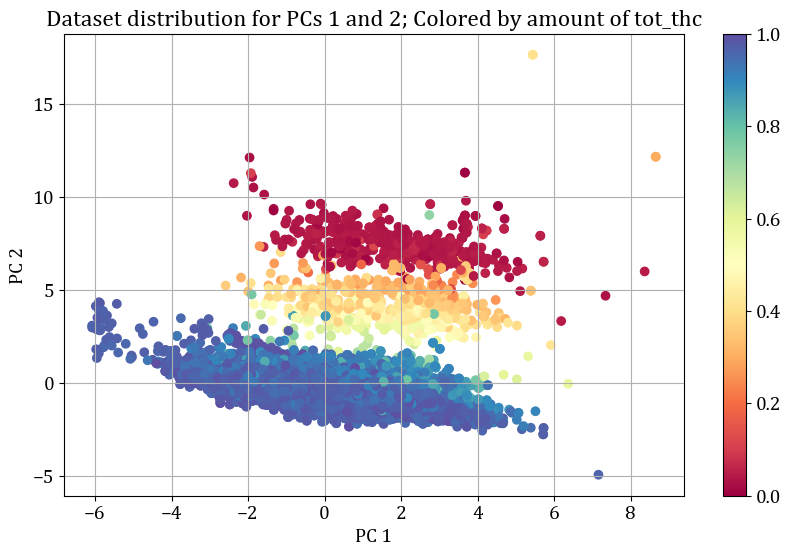
\includegraphics[width=\textwidth]{images/pc_1_2_tot_thc.png}
         \caption{Dataset distribution colored by the amount of \texttt{tot\_thc}}
         \label{fig:tot_thc}
     \end{subfigure}
     \hfill
     \begin{subfigure}[b]{0.475\textwidth}
         \centering
         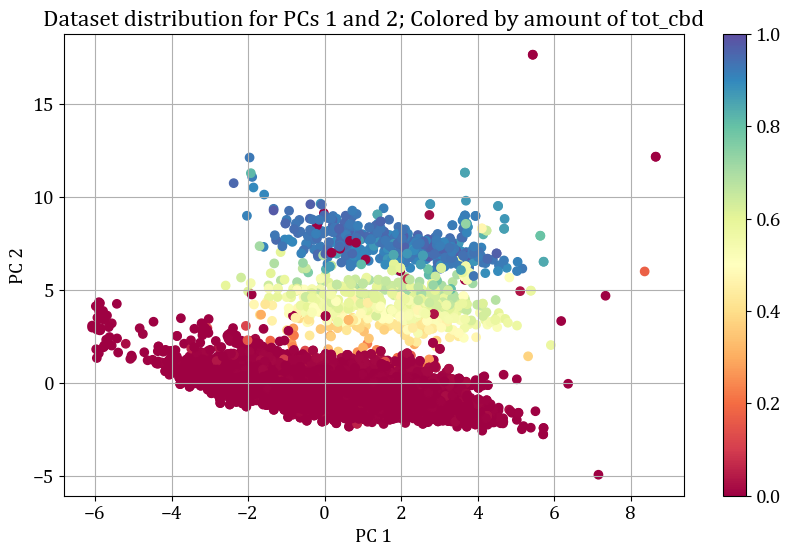
\includegraphics[width=\textwidth]{images/pc_1_2_tot_cbd.png}
         \caption{Dataset distribution colored by the amount of \texttt{tot\_cbd}}
         \label{fig:tot_cbd}
     \end{subfigure}
    \caption{Distribution of Cannabis Dataset in PC1-PC2 Space. The plot allows for visualizing the grouping and dispersion of samples in relation to the levels of THC and CBD content, respectively.}
    \label{fig:thc_cbd}
\end{figure}

\begin{figure}[H]
	\centering
	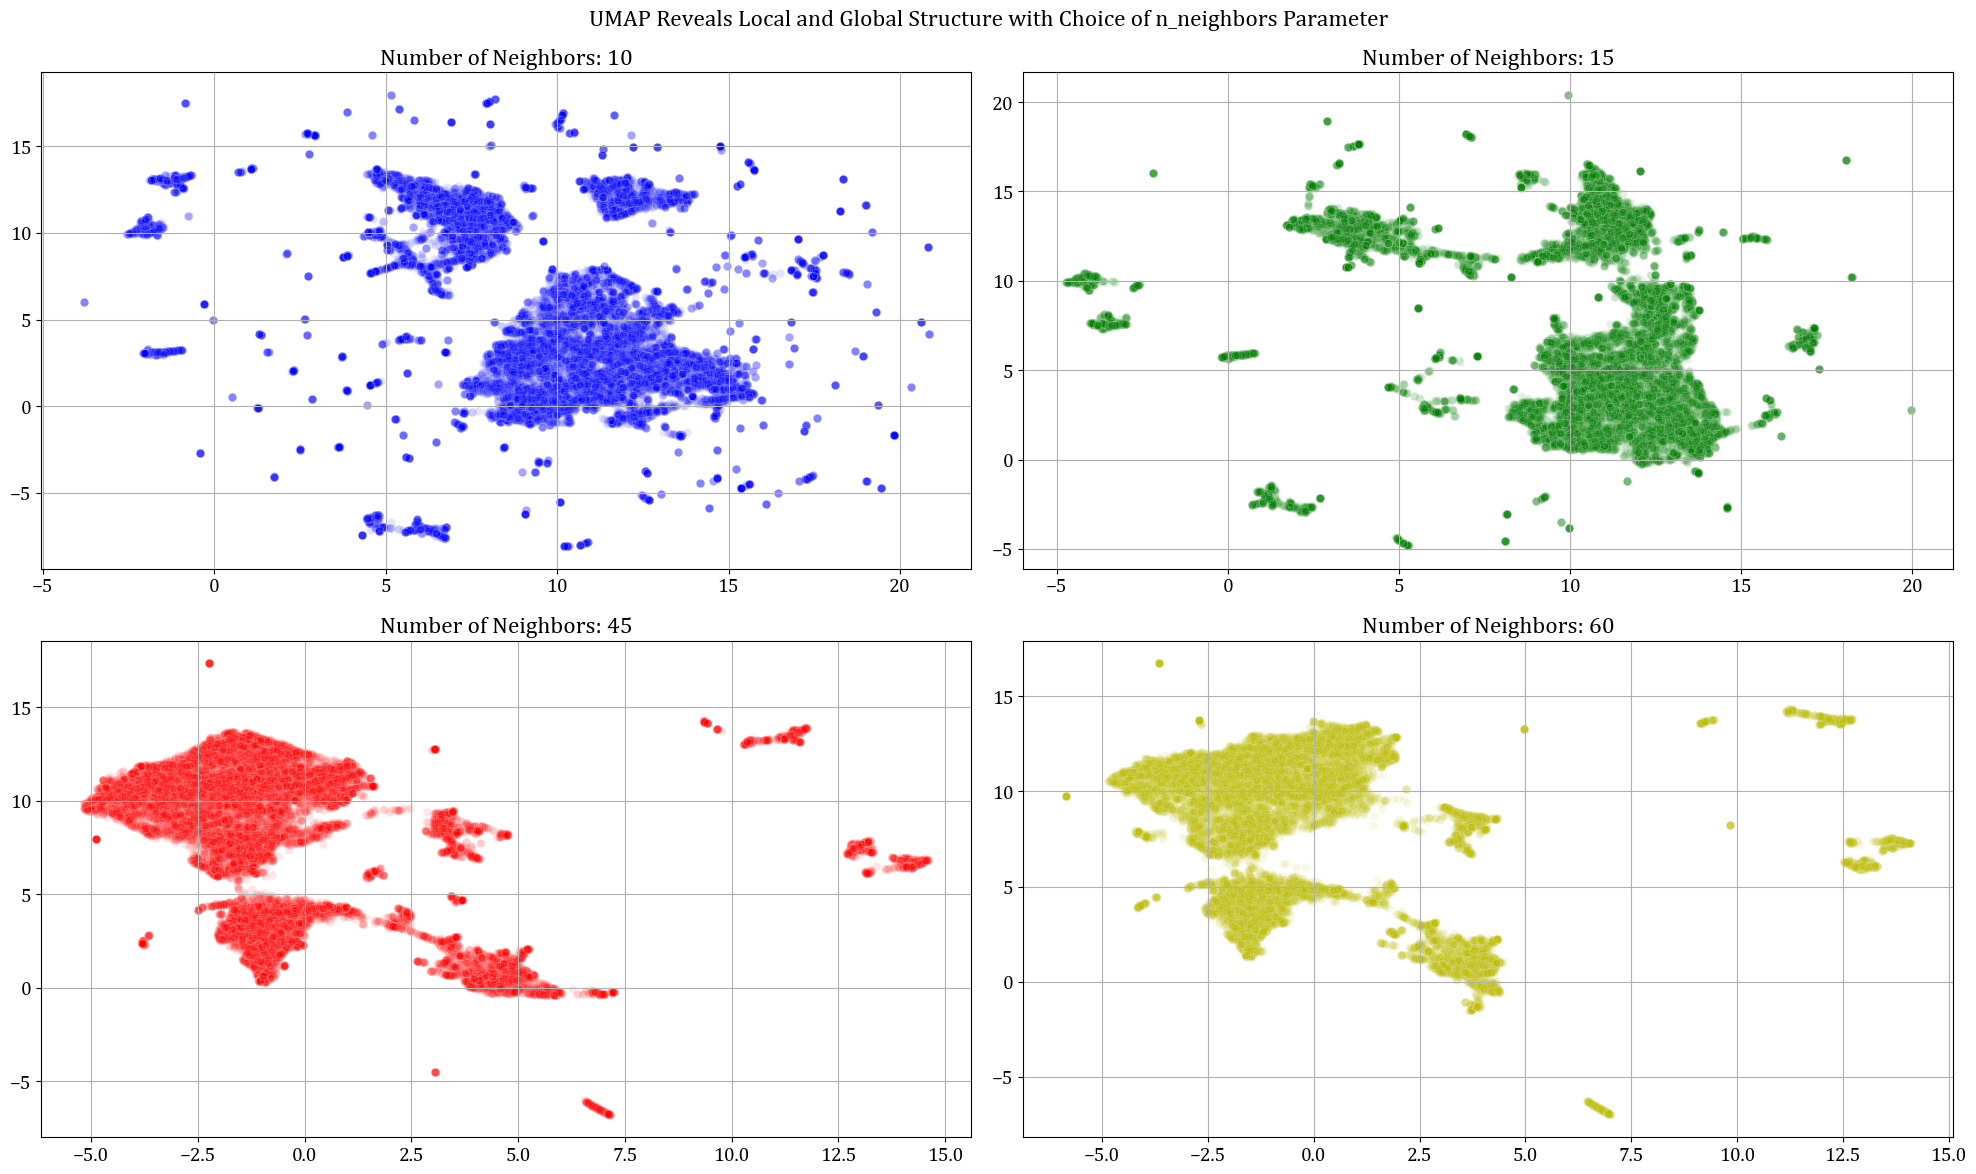
\includegraphics[scale=0.2]{images/umap_n_neighbors.png}
	\caption{UMAP Visualization with Varying Number of Neighbors. Improvements in the clustering structure becomes noticeable at 45 but further increasing the number of neighbors did not lead to further refinement in the UMAP visualization.}
	\label{fig:umap_n_neigh}
\end{figure}

\begin{figure}[H]
	\centering
	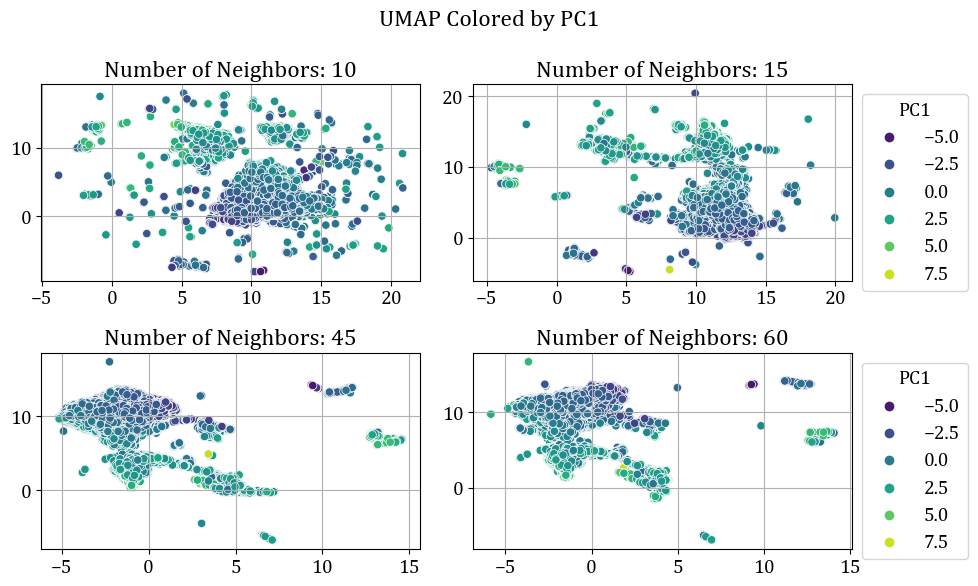
\includegraphics[scale=0.5]{images/umap_pc1.png}
	\caption{UMAP visualization of the dataset colored by Principal Component 1 (PC1).}
	\label{fig:umap_pc1}
\end{figure}

\begin{figure}[H]
	\centering
	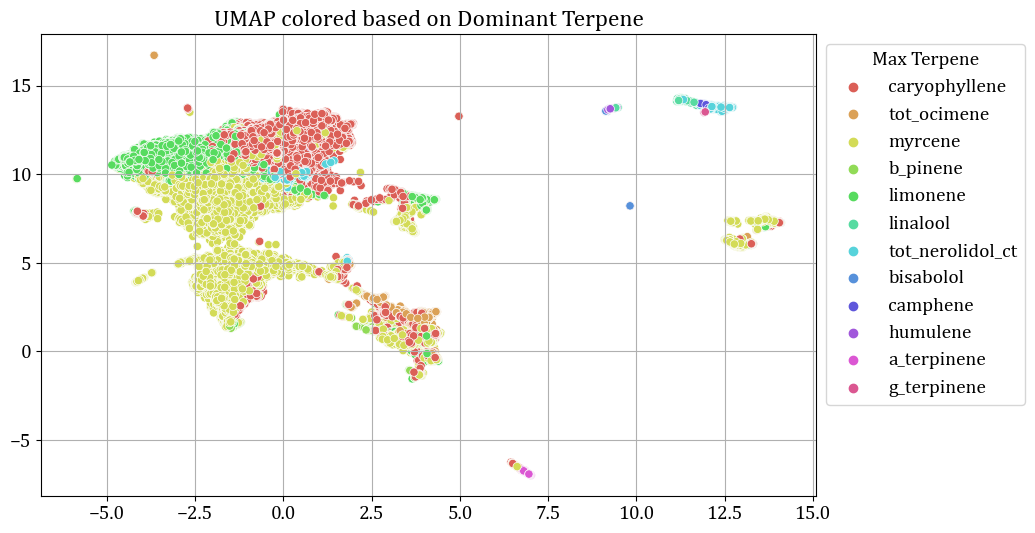
\includegraphics[scale=0.45]{images/umap_terpene.png}
	\caption{UMAP visualization of the cannabis samples colored by the dominant terpene. The plot exhibits a diverse distribution of colors, representing various dominant terpenes present in the dataset.}
	\label{fig:umap_terpene}
\end{figure}


\begin{figure}[H]
     \centering
     \begin{subfigure}[b]{0.475\textwidth}
         \centering
         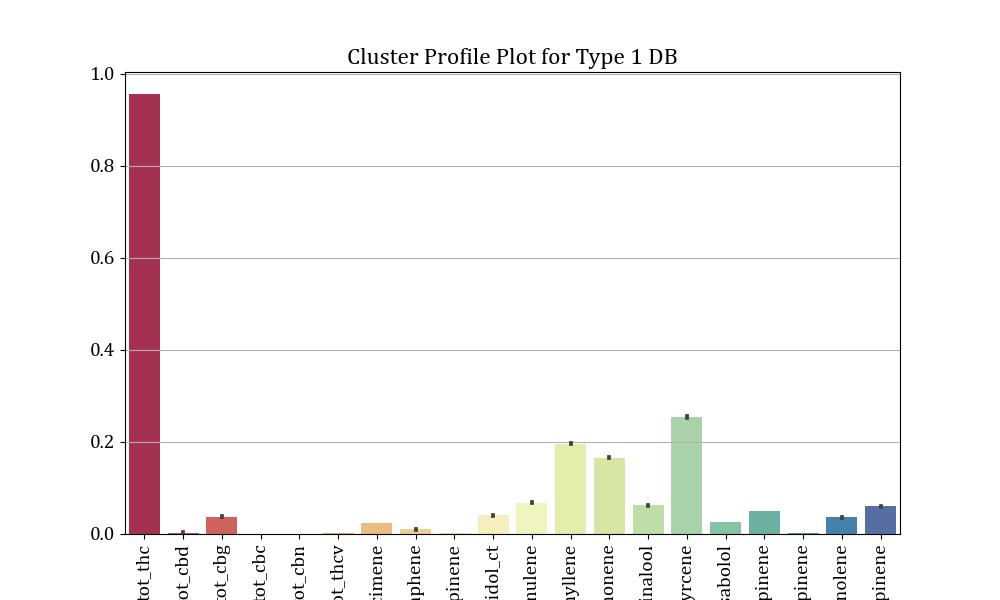
\includegraphics[width=\textwidth]{images/db_chem_composition_1.png}
         \label{fig:db_clust_1}
     \end{subfigure}
     \hfill
     \begin{subfigure}[b]{0.475\textwidth}
         \centering
         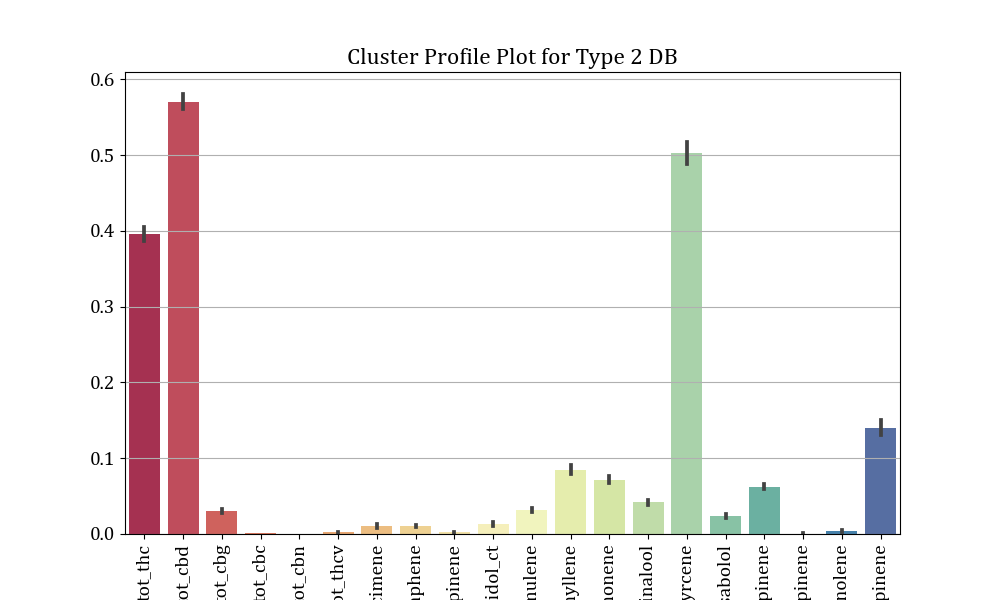
\includegraphics[width=\textwidth]{images/db_chem_composition_2.png}
         \label{fig:db_clust_2}
     \end{subfigure}
     \hfill
     \begin{subfigure}[b]{0.475\textwidth}
         \centering
         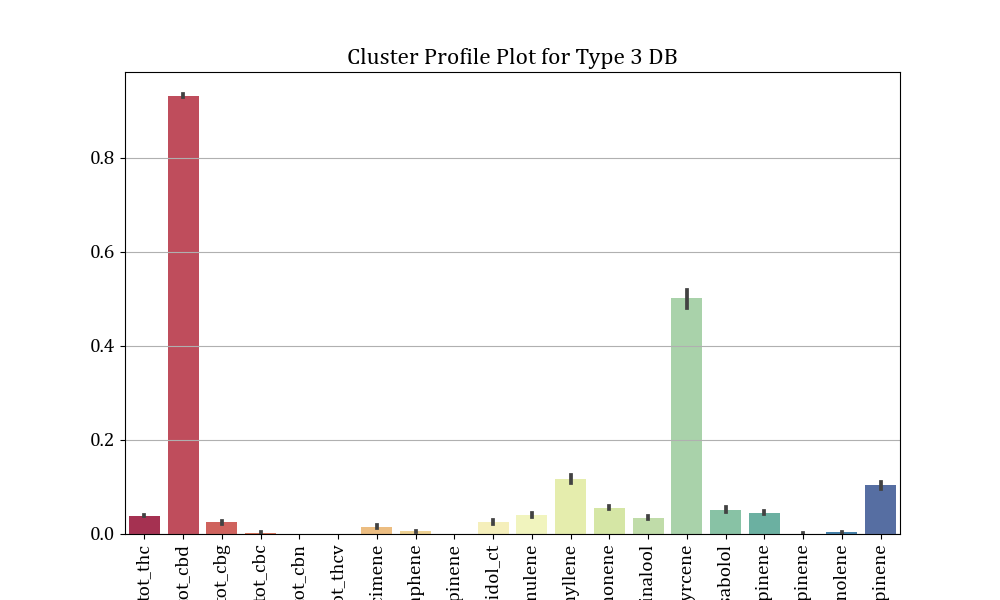
\includegraphics[width=\textwidth]{images/db_chem_composition_3.png}
         \label{fig:db_clust_3}
     \end{subfigure}
     \hfill
     \begin{subfigure}[b]{0.475\textwidth}
         \centering
         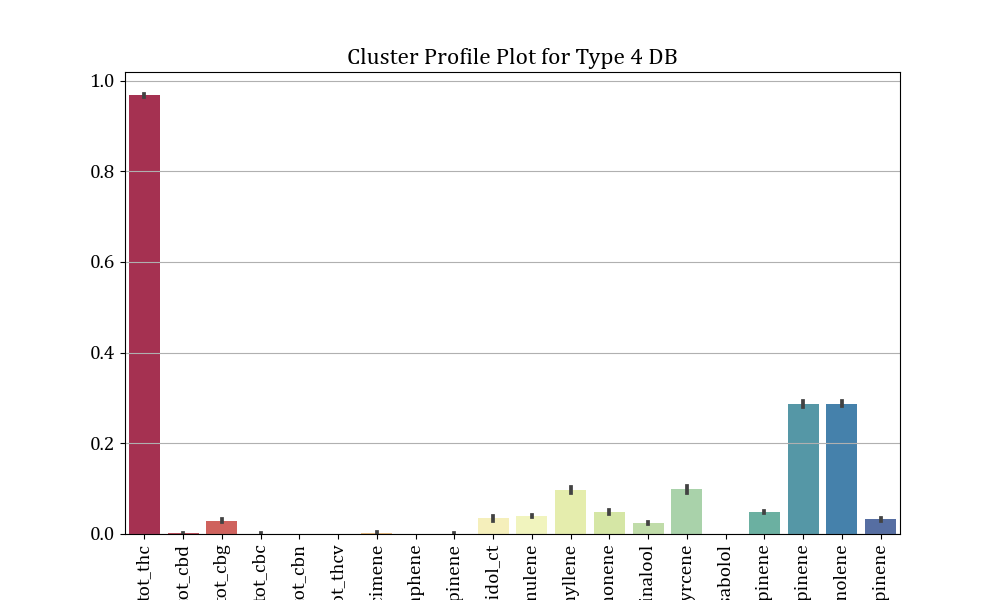
\includegraphics[width=\textwidth]{images/db_chem_composition_4.png}
         \label{fig:db_clust_4}
     \end{subfigure}
    \caption{Chemical Composition of the data points constituting DBSCAN clusters. Error bars indicate 95\% confidence intervals.}
    \label{fig:dbscan_cc}
\end{figure}


\begin{figure}[H]
     \centering
     \begin{subfigure}[b]{0.475\textwidth}
         \centering
         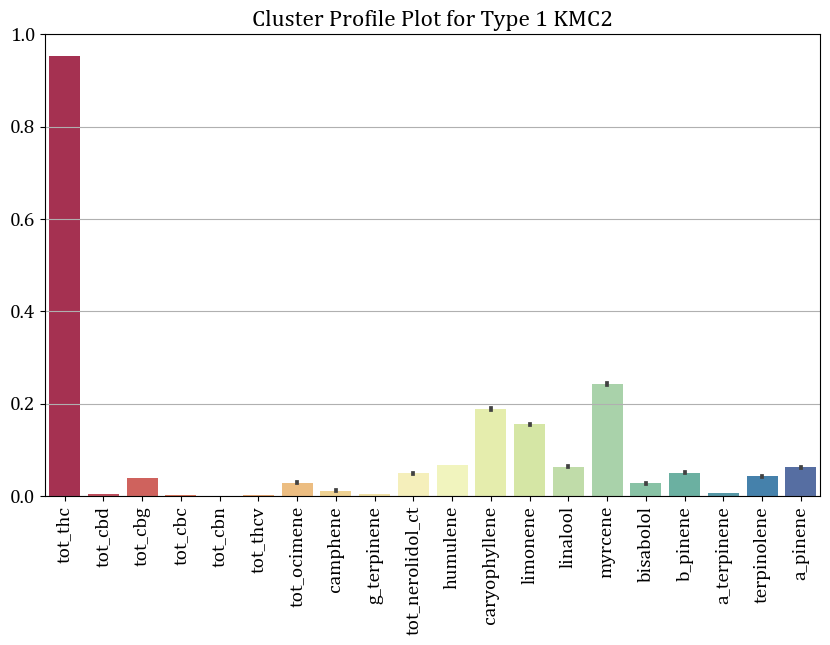
\includegraphics[width=\textwidth]{images/km2_1.png}
         \label{fig:km2_1}
     \end{subfigure}
     \hfill
     \begin{subfigure}[b]{0.475\textwidth}
         \centering
         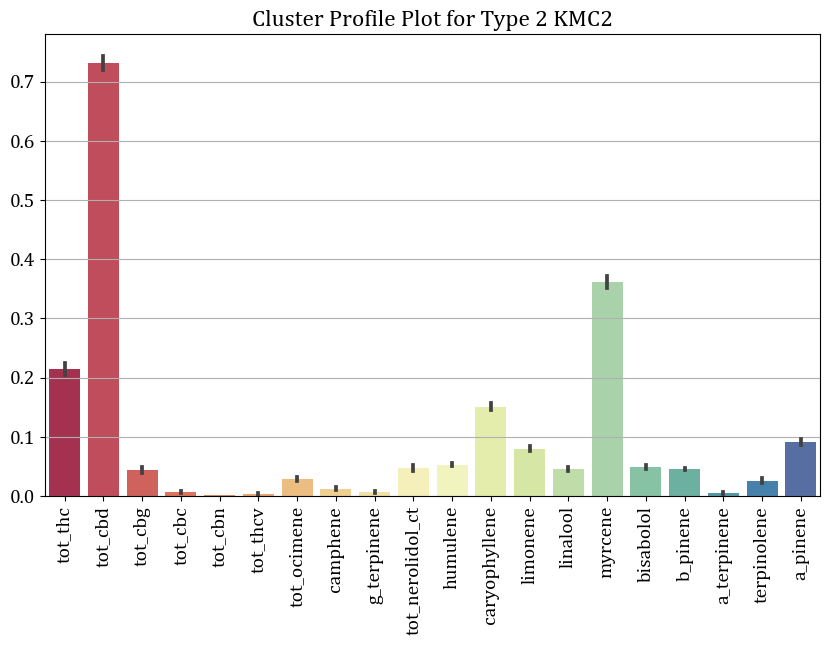
\includegraphics[width=\textwidth]{images/km2_2.png}
         \label{fig:km2_2}
     \end{subfigure}
    \caption{Chemical Composition of the data points constituting K-Means clusters with $k=2$. Error bars indicate 95\% confidence intervals.}
    \label{fig:km2}
\end{figure}

\begin{figure}[H]
     \centering
     \begin{subfigure}[b]{0.475\textwidth}
         \centering
         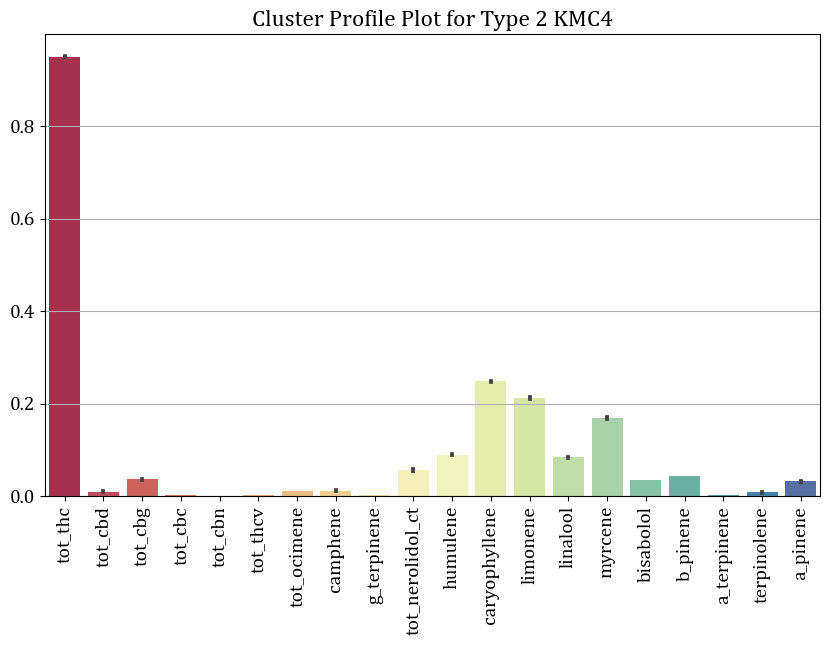
\includegraphics[width=\textwidth]{images/km4_2.png}
         \label{fig:km4_2}
     \end{subfigure}
     \hfill
     \begin{subfigure}[b]{0.475\textwidth}
         \centering
         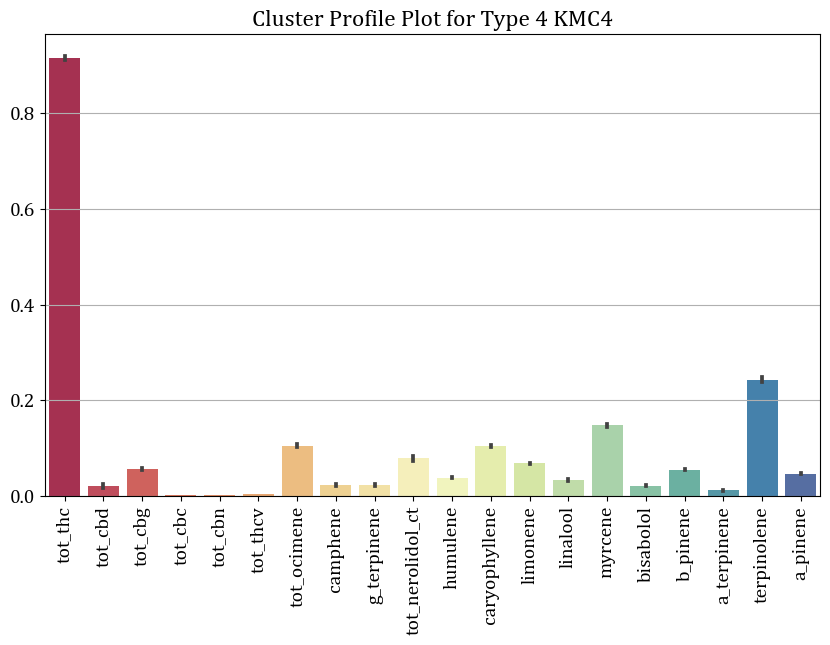
\includegraphics[width=\textwidth]{images/km4_4.png}
         \label{fig:km4_4}
     \end{subfigure}
    \caption{Chemical Composition of the data points constituting K-Means clusters with $k=4$, of clusters 2 and 4. Error bars indicate 95\% confidence intervals.}
    \label{fig:km4}
\end{figure}

\begin{figure}[H]
     \centering
     \begin{subfigure}[b]{0.475\textwidth}
         \centering
         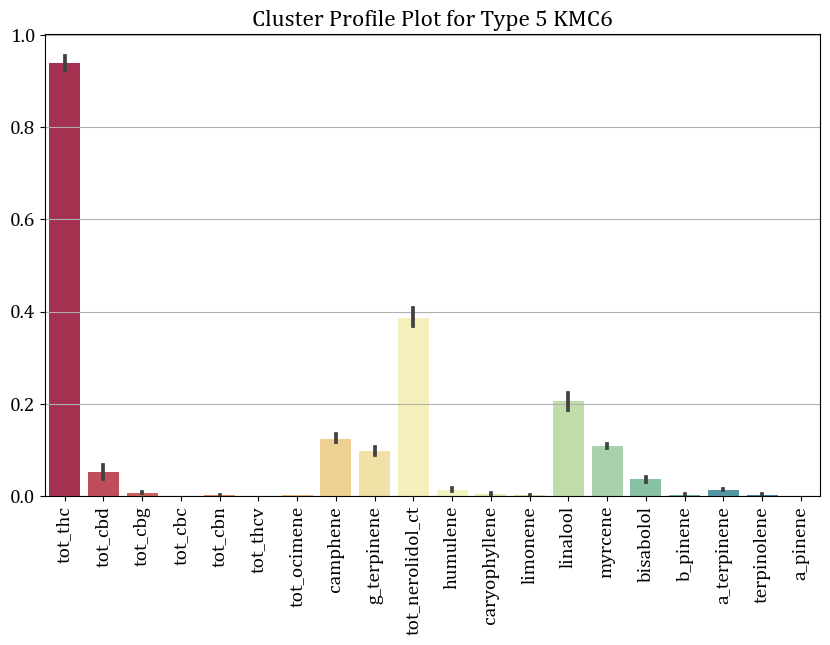
\includegraphics[width=\textwidth]{images/km6_5.png}
         \label{fig:km6_5}
     \end{subfigure}
     \hfill
     \begin{subfigure}[b]{0.475\textwidth}
         \centering
         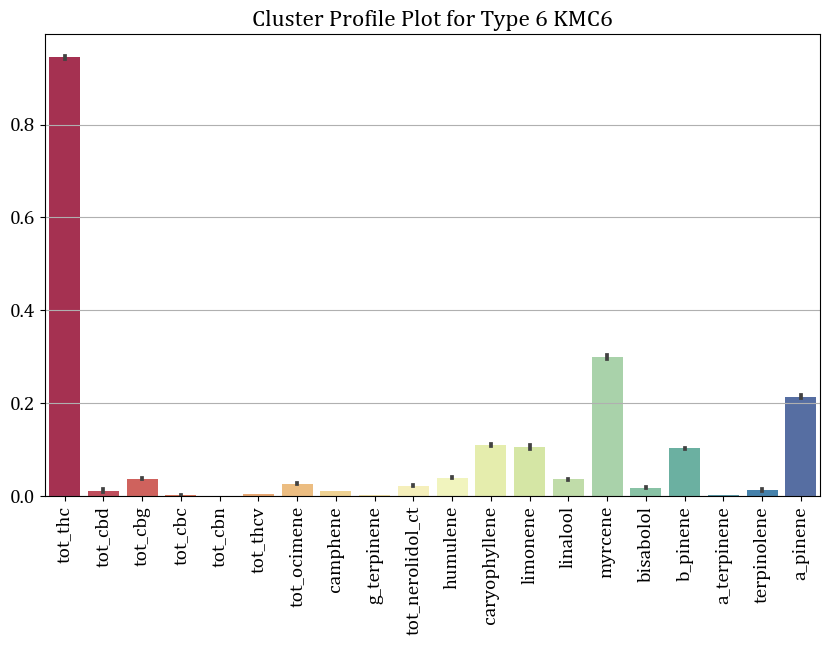
\includegraphics[width=\textwidth]{images/km6_6.png}
         \label{fig:km6_6}
     \end{subfigure}
    \caption{Chemical Composition of the data points constituting K-Means clusters with $k=6$, of cluster 5 and 6. Error bars indicate 95\% confidence intervals.}
    \label{fig:km6}
\end{figure}

\begin{figure}[H]
     \centering
     \begin{subfigure}[b]{0.475\textwidth}
         \centering
         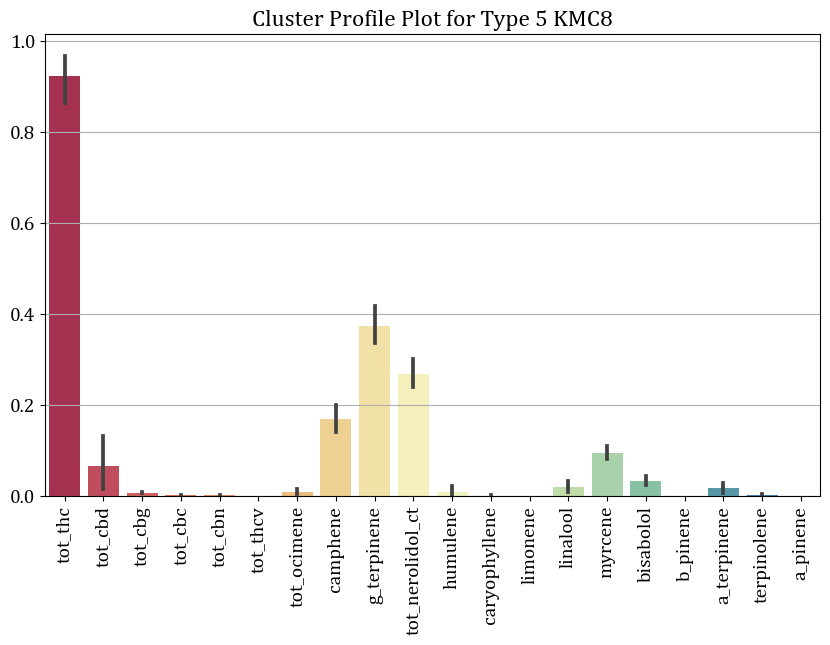
\includegraphics[width=\textwidth]{images/km8_5.png}
         \label{fig:km8_5}
     \end{subfigure}
     \hfill
     \begin{subfigure}[b]{0.475\textwidth}
         \centering
         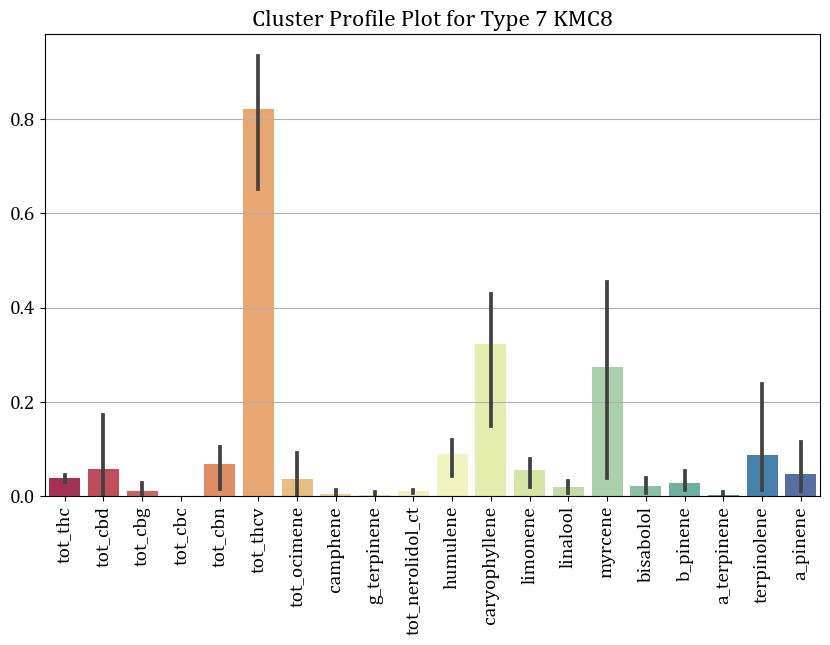
\includegraphics[width=\textwidth]{images/km8_7.png}
         \label{fig:km8_7}
     \end{subfigure}
    \caption{Chemical Composition of the data points constituting K-Means clusters with $k=8$, of cluster 5 and 7. Error bars indicate 95\% confidence intervals.}
    \label{fig:km8}
\end{figure}

\section{Discussion}
This study used two clustering algorithms for the classification of cannabis strains. Our results reveal exciting insights into the relationship between different variables and their impact on cannabis clustering principal component 1 (PC1), which captured the vast majority of the variance. This affirmed that PC1 would determine our samples' overall structure and grouping. On the other hand, principal component 2 (PC2) did not contribute significantly to dataset variance and likely had a minimal contribution to our clustering analysis.\\

\noi
We leveraged DBSCAN representation by different variables, such as regions and dominant terpenes. The acquired outcomes show that DBSCAN effectively recognized and appropriately labeled outlier data points as noise. Moreover, alongside noise detection, DBSCAN demonstrated the capability to group points exhibiting comparable chemical composition. Interestingly, when visualizing the dataset using UMAP based on regions, we did not observe clear boundaries or distinct groupings. This suggests that the regional factor alone may not be a strong predictor of the underlying structure in our dataset. Other factors or interactions between variables may play a more prominent role in shaping the observed patterns. In contrast, when utilizing UMAP based on dominant terpenes, we identified clear and dominant groups within the dataset. This finding implies that specific terpenes exert a more substantial influence on the overall structure and grouping of samples than regional distinctions. Dominant terpenes likely contribute to forming distinct clusters, suggesting their potential importance in characterizing and differentiating samples within our dataset. Our results underscore the significance of selecting the appropriate variables and considering their respective contributions when applying UMAP analysis. The choice of principal components can significantly impact the captured variance and the resulting representation. Moreover, our findings demonstrate the varying influence of different variables, such as regions and dominant terpenes, on our dataset's observed patterns and structures.\\

\noi
The results obtained for k-means clustering varied depending on the number of clusters initiated. For k-means with 2 clusters, most data points were classified in one class, while the second class contained outliers. Cluster 1 had a chemical composition similar to class 1 of DBSCAN, possibly due to k-means assigning most points to cluster 1. When using 4 clusters, k-means showed centroid-based clustering with spatially close data points in each cluster. Cluster 1 and cluster 1 from DBSCAN had a similar composition, but myrcene concentration was higher in k-means. Cluster 3 resembled cluster 4 from DBSCAN. Cluster 2 had a novel composition high in THC and caryophyllene, while cluster 4 had high THC and terpinolene but low terpinene. With 6 clusters, there was overlap between clusters, suggesting differentiation in higher-dimensional data. Composition similarities between cluster 1 and DBSCAN's cluster 1 were found, but myrcene concentration was higher in k-means. Cluster 3 resembled cluster 4 from DBSCAN. Clusters 2 and 4 were similar to the 4-cluster k-means model. Clusters 5 and 6 had novel compositions. When using 8 clusters, clusters 1-4, 6, and 8 were like previous DBSCAN or k-means models. Clusters 5 and 7 had novel compositions, with cluster 5 high in THC, g-terpinene, camphene, and nerolidol, and cluster 7 low in THC but high in THCV, myrcene, and caryophyllene. Overall, the results showed that the choice of the number of clusters influenced the classification and chemical compositions obtained through k-means clustering. Some clusters were consistent across different models, while others had unique chemical compositions.\\

\noi
Traditionally, cannabis strains have been classified based on their chemical composition, primarily the presence and relative abundance of cannabinoids, such as THC and CBD \cite{atakan2012cannabis}. However, terpenes, which are aromatic compounds found in many plants, including cannabis, have gained recognition for their potential influence on the effects and therapeutic properties of different strains. Terpenes contribute to the distinct aroma and flavor profiles of cannabis strains and are believed to work synergistically with cannabinoids. As a result, terpenes are now considered an additional factor in strain classification. By analyzing the terpene composition, researchers aim to identify patterns that could help classify strains and predict their potential effects. This approach has led to terpene-focused strain categorizations, where strains are grouped based on their dominant terpenes. Our findings from DBSCAN and K-means support the growing evidence suggesting that terpenes are a crucial factor in cannabis strain classification \cite{hanuvs2020terpenes}. Utilizing UMAP based on dominant terpenes allowed us to identify clear and dominant groups within our dataset. In contrast, UMAP based on the region of origin did not exhibit the same level of distinctiveness. These results highlight the importance of considering terpenes when developing classification systems for cannabis strains and provide valuable insights for consumers, producers, and researchers.\\

\noi
Recognizing the differences in the underlying principles and assumptions of K-means and DBSCAN is essential. K-means is a centroid-based algorithm that assumes spherical clusters and assigns each data point to the nearest centroid. On the other hand, DBSCAN is a density-based algorithm that identifies clusters based on local density variations, allowing for more irregularly shaped clusters and the ability to detect outliers. DBSCAN provides additional insights by identifying noise points and implicitly capturing density-based structures. DBSCAN's ability to detect outliers and identify denser regions could be valuable for detecting rare or unique strains that may not fit neatly into the established clusters.\\

\noi
While the K-means and DBSCAN clustering results provide valuable insights into the classification of cannabis strains, several avenues for future research and certain limitations should be considered. Firstly, the stability and generalizability of the clustering results across different datasets or sampling variations need to be assessed. Conducting cross-validation studies using independent datasets or incorporating data from different sources would enhance the reliability and robustness of the identified clusters. It is essential to acknowledge that clustering algorithms, including K-means and DBSCAN, are sensitive to the initial parameters and assumptions made during analysis. Exploring different parameter settings and comparing the results obtained from alternative clustering algorithms, such as hierarchical clustering or Gaussian mixture models, can provide a more comprehensive assessment of the cannabis dataset's structure.\\

\noi
Furthermore, it is crucial to recognize the potential limitations of the dataset itself. The quality and completeness of the data, including potential missing values or measurement errors, can impact the clustering outcomes and subsequent interpretations. Addressing these data limitations and ensuring the availability of comprehensive and reliable information would improve the accuracy and validity of the strain classification results. Lastly, while clustering algorithms offer insights into the inherent structure of the cannabis dataset, it is crucial to integrate additional information and domain expertise for a holistic understanding of strain classification. Incorporating expert knowledge, such as botanical information, historical lineage, or consumer preferences, can provide a more nuanced and comprehensive classification framework. Overall, future research endeavors should focus on further validating and refining the identified clusters, exploring different clustering algorithms and parameter settings, addressing data limitations, and incorporating domain expertise to enhance the accuracy and applicability of cannabis strain classification methods.\\

\noi
The comparison of K-means and DBSCAN clustering results highlights the effectiveness of both algorithms in classifying cannabis strains. Future studies could explore the characteristics and attributes contributing to the clustering results and further validate the identified clusters against known strains or chemical compositions. Additionally, investigating the stability and generalizability of the clustering results across different datasets or sampling variations would enhance confidence in the findings. By considering both approaches, researchers and practitioners can comprehensively understand the cannabis dataset and make informed decisions for strain classification, product development, and market segmentation.


\bibliographystyle{apalike}
\bibliography{references}

\end{document}